\vspace{1.5cm}

El detalle del cálculo del punto de reposo se realiza en la sección~\sectref{qpoint}, en la figura~\figref{fig:fig_calculated_qpoint} se muestra lo calculado.


\begin{figure}[H] %htb
\begin{center}
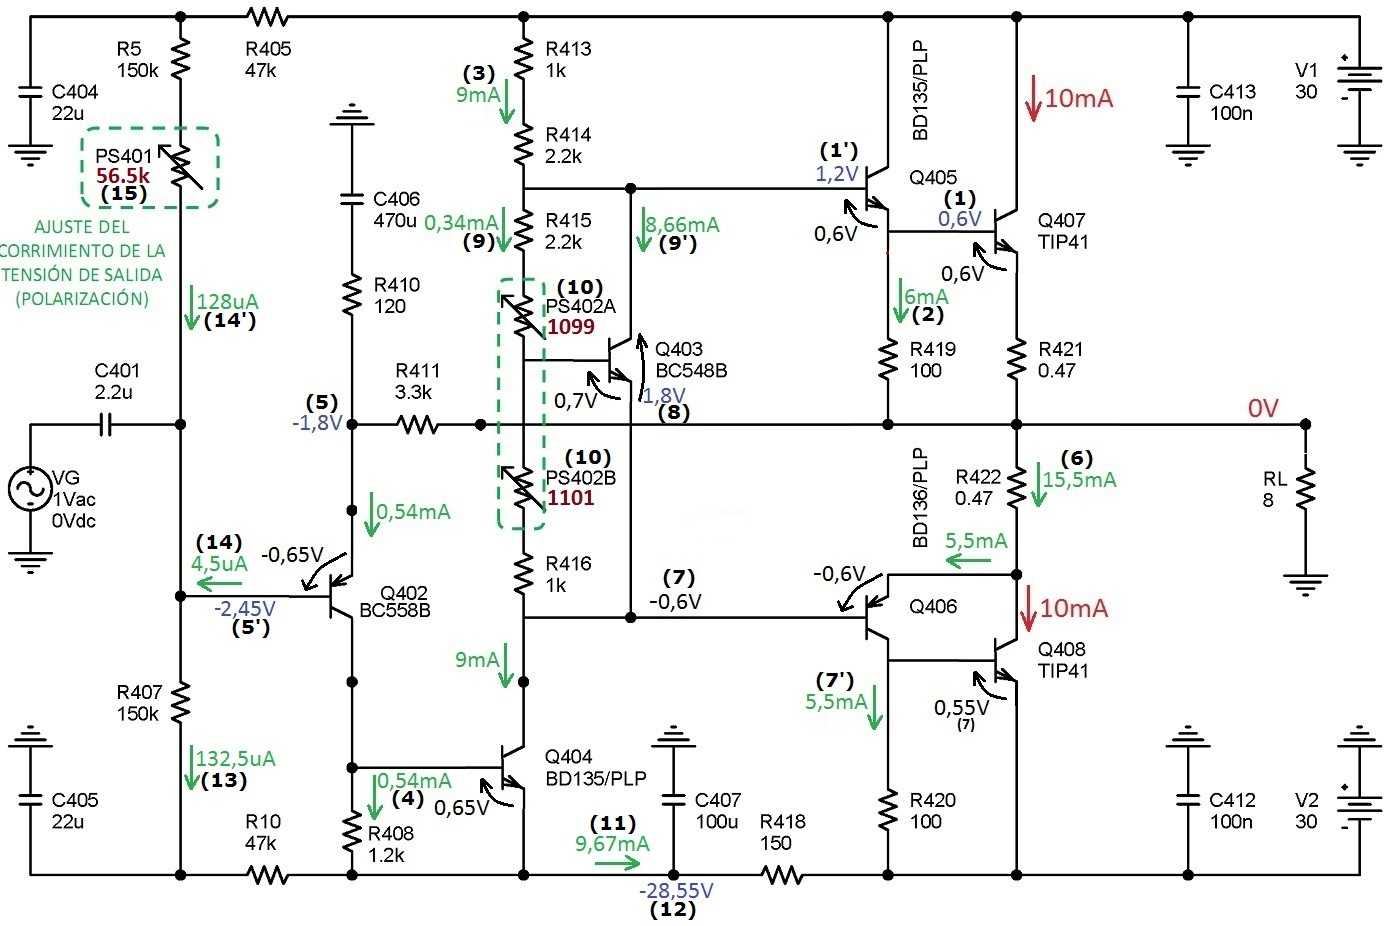
\includegraphics[width=0.9 \textwidth, angle=0]{./img/qpoint/polarizacion_calculada.png}
\caption{\label{fig:fig_calculated_qpoint}\footnotesize{Punto de reposo del circuito.}}
\end{center}
\end{figure}


\vfill

\clearpage
